\documentclass[
	a4paper, % Paper size, use either a4paper or letterpaper
	10pt, % Default font size, can also use 11pt or 12pt, although this is not recommended
	unnumberedsections, % Comment to enable section numbering
	twoside, % Two side traditional mode where headers and footers change between odd and even pages, comment this option to make them fixed
]{LTJournalArticle}

\usepackage{lettrine}
\usepackage{subcaption}
\usepackage{graphicx}
\usepackage{float}
\usepackage{booktabs}
\usepackage{tikz}
\usetikzlibrary{positioning}

\addbibresource{references.bib} % BibLaTeX bibliography file

\runninghead{3D Reconstruction with Gaussian Splatting: A Review} % A shortened article title to appear in the running head, leave this command empty for no running head

\footertext{} % Text to appear in the footer, leave this command empty for no footer text

\setcounter{page}{1} % The page number of the first page, set this to a higher number if the article is to be part of an issue or larger work

%----------------------------------------------------------------------------------------
%	TITLE SECTION
%----------------------------------------------------------------------------------------

\title{3D Reconstruction with Gaussian Splatting: A Review} % Article title, use manual lines breaks (\\) to beautify the layout

% Authors are listed in a comma-separated list with superscript numbers indicating affiliations
% \thanks{} is used for any text that should be placed in a footnote on the first page, such as the corresponding author's email, journal acceptance dates, a copyright/license notice, keywords, etc
\author{%
	Christian Faccio\textsuperscript{1} \thanks{\href{mailto:christianfaccio@outlook.it}{christianfaccio@outlook.it}}, 
    Elena Lorite\textsuperscript{1} \thanks{\href{mailto:elenalorite@gmail.com}{elenalorite@gmail.com}} and
    Jorge Huedo Martínez\textsuperscript{1} \thanks{\href{mailto:jhm31@alu.ua.es}{jhm31@alu.ua.es}} 
}

% Affiliations are output in the \date{} command
\date{\footnotesize\textsuperscript{\textbf{1}}University of Alicante}

% Full-width abstract
\renewcommand{\maketitlehookd}{%
	\begin{abstract}
		\noindent 3D scene reconstruction from multiple views is a long-standing problem in computer vision, and the recent introduction of 3D Gaussian Splatting (3DGS) has reshaped the field by combining the rendering quality of Neural Radiance Fields with real-time inference and a fully explicit scene representation. In this work we review the state of the art of multi-view 3D reconstruction methods centred on the Gaussian Splatting paradigm. We first place 3DGS in context by surveying the photogrammetry and Structure-from-Motion pipelines that precede it and the Neural Radiance Field family that motivated it, as well as 3D-Free alternative pipelines, then describe the core 3DGS algorithm in detail, including the 3D-to-2D Gaussian projection, the Adaptive Density Control schedule and the tile-based rasteriser that makes real-time rendering possible. We then discuss recent applications of 3DGS in autonomous driving, bi-modal RGB-IR mapping, in-the-wild urban surveying, super-resolution and sparse-view reconstruction, and digital twins for infrastructure inspection. We complete the review with a brief overview of the datasets that have become standard benchmarks for the technique, and a small reproduction experiment in which we run the official 3DGS implementation on the \texttt{bonsai} scene of the Mip-NeRF 360 dataset using a free Colab T4 GPU. Our run matches the quality numbers reported in the original paper to within run-to-run variance, while incurring a $\sim 2$--$3.5\times$ slowdown in training and inference, confirming that 3DGS scales gracefully down to commodity hardware without sacrificing rendering quality.
	\end{abstract}
}

%----------------------------------------------------------------------------------------

\begin{document}

\maketitle % Output the title section

%----------------------------------------------------------------------------------------
%	ARTICLE CONTENTS
%----------------------------------------------------------------------------------------

\section{Introduction}
\lettrine[findent=2pt]{\textbf{I}}{}n the field of Computer Vision, 3D scene and object reconstruction from multiple views is the task in which the geometrical structure of a scene is inferred from a collection of images. The objective is to solve a pixel-wise correspondence problem from these images, assuming or estimating the position of the cameras and the internal parameters \cite{tum_mvr}.
Although being one of the most fundamental problems in the field, it still poses several challenges. Different methods exist, each with different representations and outputs, and with their own compromises in speed, complexity or accuracy \cite{review_3drecon_2025}. Over the years, new advances have been achieved, proposing methodologies able to perform real time and detailed reconstructions of 3D scenes; one of these methodologies is Gaussian Splatting, which uses 3D Gaussians with Structure-from-Motion (SfM) inputs \cite{kerbl20233dgs}. In broader terms, it represents the scene as a cloud of 3D Gaussian points, enabling efficient and realistic visualization with effects like transparency and anti-aliasing.
In this work, we review the state of the art of the methods that address the problem of multiview 3D scene reconstruction using the Gaussian Splatting technique. The document is structured as follows: Section 2 introduces the literature previous to Gaussian Splatting and the basis behind the Gaussian Splatting technique. Section 3 explains the details behind the Gaussian Splatting methodology as well as a discussion of its performance and other extensions of the technique. Section 4 explores different applications of the Gaussian Splatting technique in other works. Section 5 performs a practical experimentation on Gaussian Splatting models for further insights. Finally, Section 6 summarises the information from the previous sections.

\section{Previous Work}
In this section, we discuss different methodologies and resources for 3D multiscene reconstruction that have been relevant in the literature of the topic. We expect to provide a general context of the field of 3D reconstruction to those readers who may not be up to date in the field as well as providing understanding on what characterises the Gaussian Splatting technique, explained in detail in Section 3.

Comprehensive surveys exist at several levels of the 3D reconstruction stack and are a useful entry point to the field: classical Structure-from-Motion pipelines are thoroughly reviewed in \cite{survey_sfm_ozyesil2017}, while \cite{survey_mvs_furukawa2015} offers a tutorial on Multi-View Stereo that complements SfM by producing dense reconstructions. For the neural side, \cite{survey_nerf_gao2022} surveys Neural Radiance Fields and, in its more recent revisions, also bridges the transition towards Gaussian-based representations. Building on these, the following subsections focus on the specific methodological threads most relevant to Gaussian Splatting.

\subsection{Photogrammetry}
Photogrammetry refers to the act of taking reliable measurements from photographs. Specifically, it relies in the idea that an object can be represented in three dimension from multiple two-dimensional images taken from different angles, following the same principles behind the stereoscopic human vision \cite{photogrammetry_2freedom}. It can be understood as an inverse process from photography: obtain a 3D model from features of 2D representations.
One of the key concepts in photogrammetry is \textbf{triangulation}: the process of identifying common points in overlapping pictures to determine its position in the 3D space, with the use of external parameters like camera position and orientation \cite{photogrammetry_artec}. Fig.~\ref{fig:1} features a diagram of this process.
In the field of computer vision, the pipeline of recovering 3D information from images is often referred as Structure-from-Motion (SfM). One benefit of SfM is that projection matrices can be computed from the corresponding points in each view \cite{sfm_medium}.

\begin{figure}
	\centering
	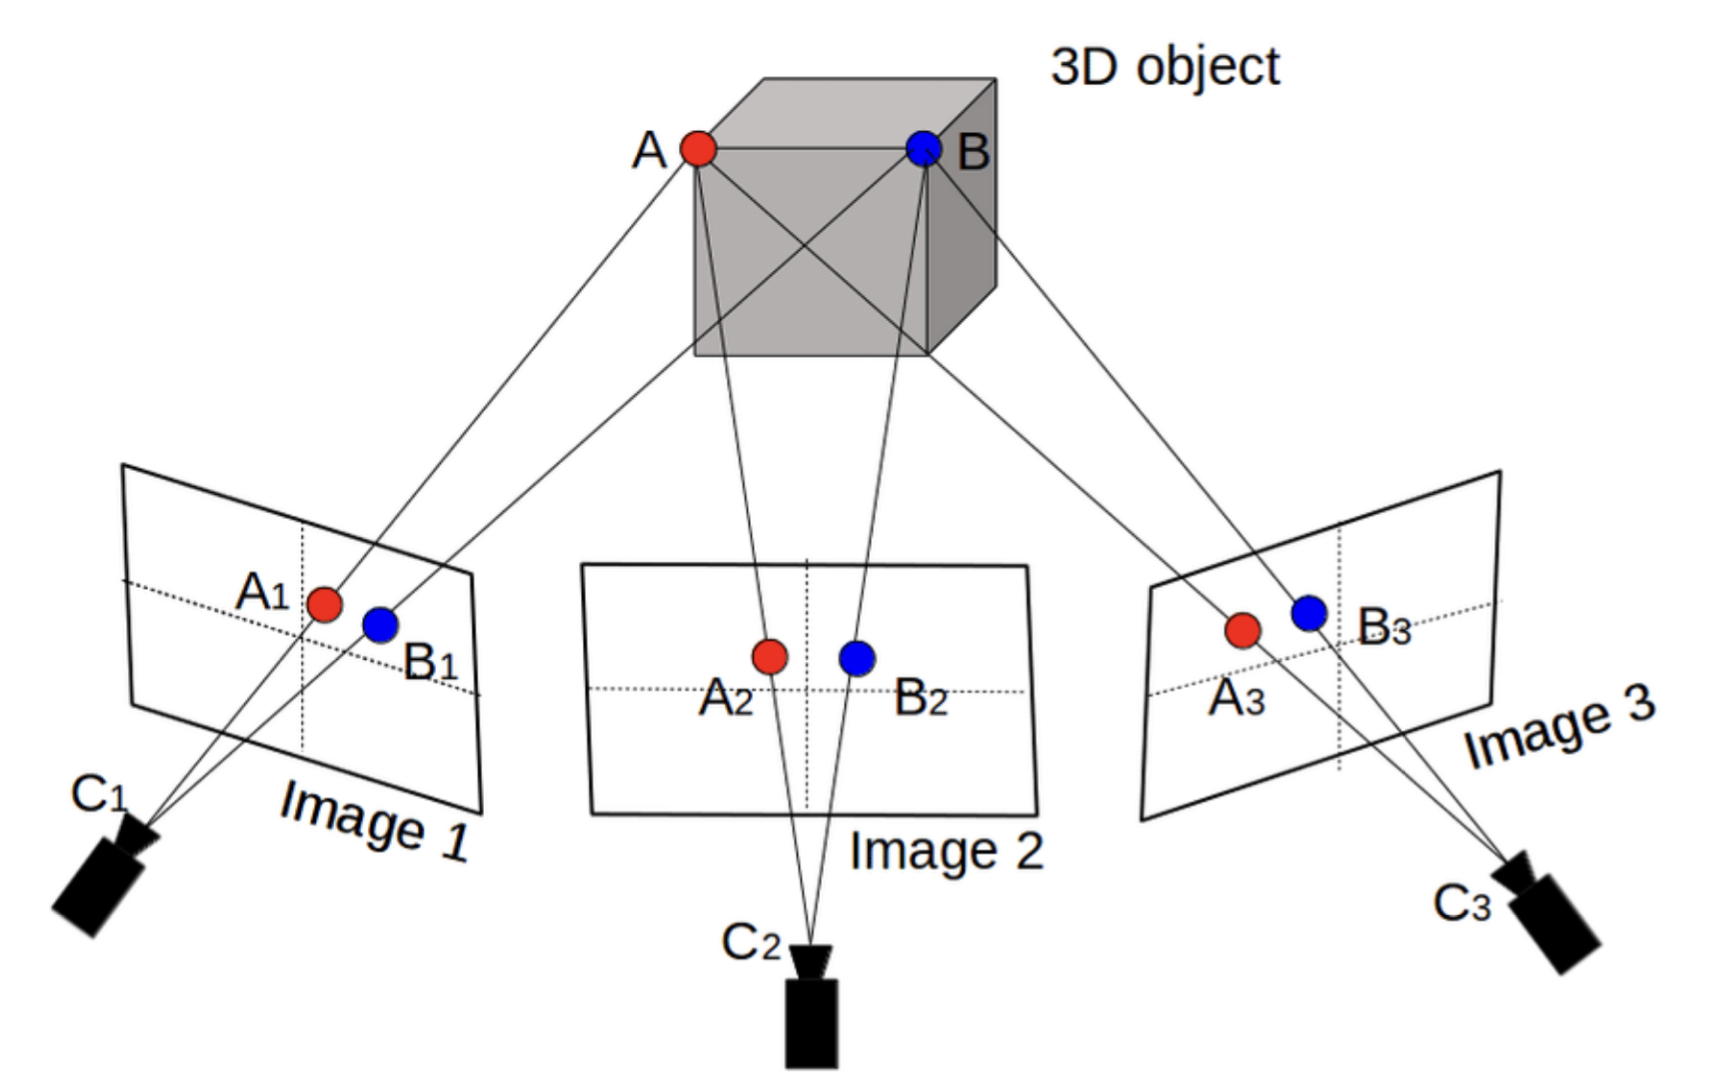
\includegraphics[width=0.45\textwidth]{assets/1.png}
	\caption{Process of triangulation in 3D reconstruction.}
	\label{fig:1}
\end{figure}

The pipeline is traditionally composed of four steps: \textit{feature extraction}, which consists on detecting local features, ideally invariant under geometric changes, from the source images; \textit{feature matching}, in which the previously obtained features are used to identify images that see the same scene part; \textit{3D reconstruction}, and finally, \textit{bundle adjustment}, in which the 3D points and camera positions are refined. However, this process can vary between works. For example in \cite{schoenberger2016sfm}, feature matching is followed by a geometric verification step that tries to estimate a transformation mapping between feature points of the images using geometric relations. In addition, 3D reconstruction is done incrementally, based on image registration from an initial two-view reconstruction and triangulation.
Since the outputs of SfM pipelines are sparse point clouds and camera positions, it is usual to apply additional techniques such as Multi-view Stereo (MVS). This method also produces a 3D model from 2D inputs, but relies on information that can be calculated by SfM such as camera parameters. MVS outputs a dense 3D representation in contrast with SfM, refining its output as a result \cite{stackoverflow_mvs_sfm}.
The MVS pipeline, as previously stated, typically uses the camera poses from SfM to estimate a depth map for each image and fuse them into the 3D point clouds. Then, volumetric 3D reconstruction is applied to construct a triangular mesh of the object \cite{romanoni2021facetwise}. 
Recently, research has drifted towards learning-based modules like DUSt3R \cite{wang2024dust3r}, which computes a stereo reconstruction for all the image pairs to obtain globally aligned pointmaps for all the cameras optimising pairs of rigid transformations and local pointmaps. Other works such as Light3R-SfM \cite{elflein2025light3rsfm} aim to directly obtain the globally aligned camera poses avoiding the global alignment step through the use of an attention module.

\subsection{Neural Radiance Fields (NeRF)}

Neural radiance fields (NeRF) represent a scene as a continuous function, mapping a position and a direction to a specific colour and volume density. NeRF models approximate this function by means of neural networks, specifically MLP, regressing from a 5D coordinate (encoding the position in the space and the direction) to the density and colour \cite{mildenhall2020nerf}. This method also utilises positional encodings to create a mapping of the input to the high frequencies, improving the resolution of the output.
Nowadays, feed-forward approaches are being proposed. As stated in \cite{feedforward_nerf_survey}, this addresses the optimisation specific for each scene which limits generalisation. From this approach, several models can be classified based on the shape of its features: 1D, 2D or 3D.
Some methods try to encode a one-dimensional vector that englobes the NeRF prediction, such as CodeNeRF \cite{jang2021codenerf}. It extends the original NeRF methodology by “learning to disentangle shape and texture by learning separate embeddings”. However, this approach requires optimisation on test time.
For 2D feature representations, models typically employ an image encoder. We can find some examples in the literature such as NerFormer \cite{reizenstein2021nerformer}. This approach employs Transformers and neural implicit rendering to learn how to reconstruct the object thanks to “jointly aggregate features from the source views”.
Finally, we could identify different types of 3D feature-based models from the type of 3D feature it uses as its representation \cite{feedforward_nerf_survey}. On one hand, models can employ 3D volume features, which are inspired by the previously mentioned MVS. A specific example of this is MVSNeRF \cite{chen2021mvsnerf}, which focuses on “learning a generic network for radiance field reconstruction”. Specifically, the radiance field is used to do regression for the rendering properties of the object, which is then used in the synthesis. On the other hand we find models that use 3D triplane features, such as the Large Reconstruction Model (LRM) \cite{hong2023lrm}. This model is based on a Transformer architecture as well, consisting of an image encoder (which encodes the input into feature tokens) and a decoder that projects such features into a triplane representation. This representation is used for NeRF prediction.

\subsection{3D-Free Models}

Contrary to other model families, 3D-Free models generate reconstructions of a scene without the aid of 3D representations like the previously introduced NeRF or Gaussian Splatting. This can be achieved with a regressive or a generative approach.

Regression methods model the reconstruction as a regression problem; a rendering function is learnt by the model to predict the pixels of a new view. Usually, this is done with transformer networks. Specific applications include Scene representation transformer (SRT) \cite{sajjadi2022scene}, which given a few images of an unseen scene, synthesises novel views, preprocessing the images via a shared CNN backbone and into patch embeddings, and processing them with a transformer encoder. Another relevant model is the Really Unposed Scene representation Transformer (RUST) \cite{sajjadi2023rustlatentneuralscene}, which completely ditches pose information, encoding the input images through a CNN and a transformer, and obtaining the target through a transformer decoder conditioned on a query. In addition to these models, we can find some approaches that use geometric information, such as Generalizable Patch-Based Neural Rendering (GPNR) \cite{suhail2022generalizablepatchbasedneuralrendering}. In this approach, linear patch embeddings are taken as input. These are then embedded and passed through a transformer network to map a light field and reference patches to radiance.

Generative methods, however, are based on using generative models to create new views from learnt data distributions. Most recent advances make use of latent diffusion models, either with image or video inputs, encoding them through a variational autoencoder \cite{feedforward_nerf_survey}. The Zero-1-to-3 framework \cite{liu2023zero1to3zeroshotimage3d} is often applied for image inputs, generating views of an object from a different angle. This is achieved building over big, pretrained models (such as Stable Diffusion), adapting them into learning camera poses and view synthesis. On the other hand, models such as GenFusion \cite{wu2025genfusionclosingloopreconstruction} align 3D reconstruction and generation through video renderings. Specifically, this approach takes advantage of a "bidirectional enhancement mechanism loop": information obtained from the generative model is used to improve reconstruction, which directly helps the generative model in producing better results.

\subsection{Datasets}

To conclude this section, we introduce a collection of datasets used for training and validating 3D reconstruction models. The aim is to provide context on what is typically found in a dataset, and to motivate the choice of dataset for the experimentation reported in Section 5.

In \cite{datasets_3drecon}, emphasis is put on how reconstruction performance can vary substantially across different scenarios, and datasets are grouped according to what they represent: human bodies, indoor scenes and outdoor scenes. We follow the same taxonomy here, but only as a brief overview, since the bulk of the discussion focuses on the datasets that have become the de-facto benchmarks for 3D Gaussian Splatting.

\textit{Human bodies.} Datasets in this category typically consist of multi-view RGB or RGB-D recordings of one or more subjects, paired with 3D body, skeleton or mesh annotations obtained from motion-capture systems. Representative examples include Human3.6M, ZJU-MoCap and the THuman series. They are used mostly for human-centric reconstruction, avatar generation and dynamic body modeling, rather than for full-scene novel view synthesis.

\textit{Indoor scenes.} These datasets capture rooms and buildings with RGB-D sensors or laser scanners and provide dense ground-truth geometry. Common examples are ScanNet, Replica and Matterport3D, which are widely used as benchmarks for indoor SLAM, surface reconstruction and semantic 3D scene understanding.

\textit{Outdoor scenes.} Outdoor datasets cover street-scale and large-scale environments captured from vehicles, drones or handheld rigs, with ground truth coming from LiDAR or terrestrial laser scanners. Representative examples include KITTI for autonomous driving scenarios, ETH3D for high-resolution multi-view stereo, and Tanks and Temples for large-scale scene reconstruction.

\textbf{Benchmarks for 3D Gaussian Splatting.} Although the datasets above span the whole 3D reconstruction landscape, the literature on 3D Gaussian Splatting has converged on a much smaller set of benchmarks, originally introduced by the seminal paper \cite{kerbl20233dgs}: Mip-NeRF 360, Tanks and Temples, Deep Blending, and the synthetic NeRF Blender dataset. Most subsequent works on 3DGS extensions, compression and applications report results on these same datasets, which makes them the natural reference for any new experiment.

\textit{Mip-NeRF 360} \cite{barron2022mipnerf360} is the most widely used 3DGS benchmark. It consists of nine real, unbounded, object-centric scenes (five outdoor and four indoor), each captured with 100--330 photographs taken on an orbital trajectory around a central object, with shared intrinsics calibrated using the OpenCV radial distortion model. Its mixture of indoor and outdoor environments and its background complexity make it a particularly challenging testbed for novel view synthesis.

\textit{Tanks and Temples} \cite{knapitsch2017tanks} is a large-scale scene reconstruction benchmark with high-resolution video captures and ground-truth point clouds acquired with an industrial laser scanner. The 3DGS paper reports results on the ``Truck'' and ``Train'' sequences, which have since become standard test scenes for 3DGS variants targeting larger environments.

\textit{Deep Blending} \cite{hedman2018deepblending} provides 19 scenes and roughly 2{,}630 photographs together with COLMAP SfM and MVS reconstructions, refined depth maps and a global textured mesh. The 3DGS paper evaluates on the ``Dr Johnson'' and ``Playroom'' scenes, which exhibit cluttered indoor geometry and view-dependent effects that stress free-viewpoint rendering methods.

\textit{NeRF Synthetic (Blender)} \cite{mildenhall2020nerf} contains synthetic, object-centric scenes rendered from Blender models. Being noise-free and fully controlled, it is mainly used for ablation studies and as a sanity-check benchmark.

Beyond these four classics, more recent datasets are starting to extend 3DGS benchmarking to capture conditions that the original benchmarks do not cover. A notable example is \textit{FIORD} \cite{fiord2025}, a fisheye indoor-outdoor dataset of ten scenes (five indoor and five outdoor) recorded with a dual 200° fisheye rig and accompanied by Faro LIDAR ground-truth point clouds. FIORD provides baseline results for vanilla 3DGS and Nerfacto, and specifically targets the wide field-of-view setting that is largely absent from Mip-NeRF 360 and Tanks and Temples.

For the experimentation reported in Section 5, we adopt \textit{Mip-NeRF 360} as the reference dataset: it contains both indoor and outdoor scenes, it is supported out of the box by virtually every 3DGS implementation, and it was used in the original 3DGS paper, which makes our results directly comparable to the published baselines.

\section{Gaussian Splatting}

\subsection{How it works}

The algorithm is composed of three main parts:
\begin{enumerate}
	\item Initialization of multiple 3D gaussians randomly
	\item Optimization of their parameters using gradient descent and Adaptive Density Control
	\item Efficient rendering using a differentiable tile-based rasterizer
\end{enumerate}

A single gaussian is defined as:
\begin{equation}
	f_i(x) = \sigma(\alpha_i)\exp^{-\frac{1}{2}(x-\mu_i)^T\Sigma_i^{-1}(x-\mu_i)}
\end{equation}

but now that we have a 3D volume composed of gaussians, how do we represent it in 2D?

\begin{figure}
	\centering
	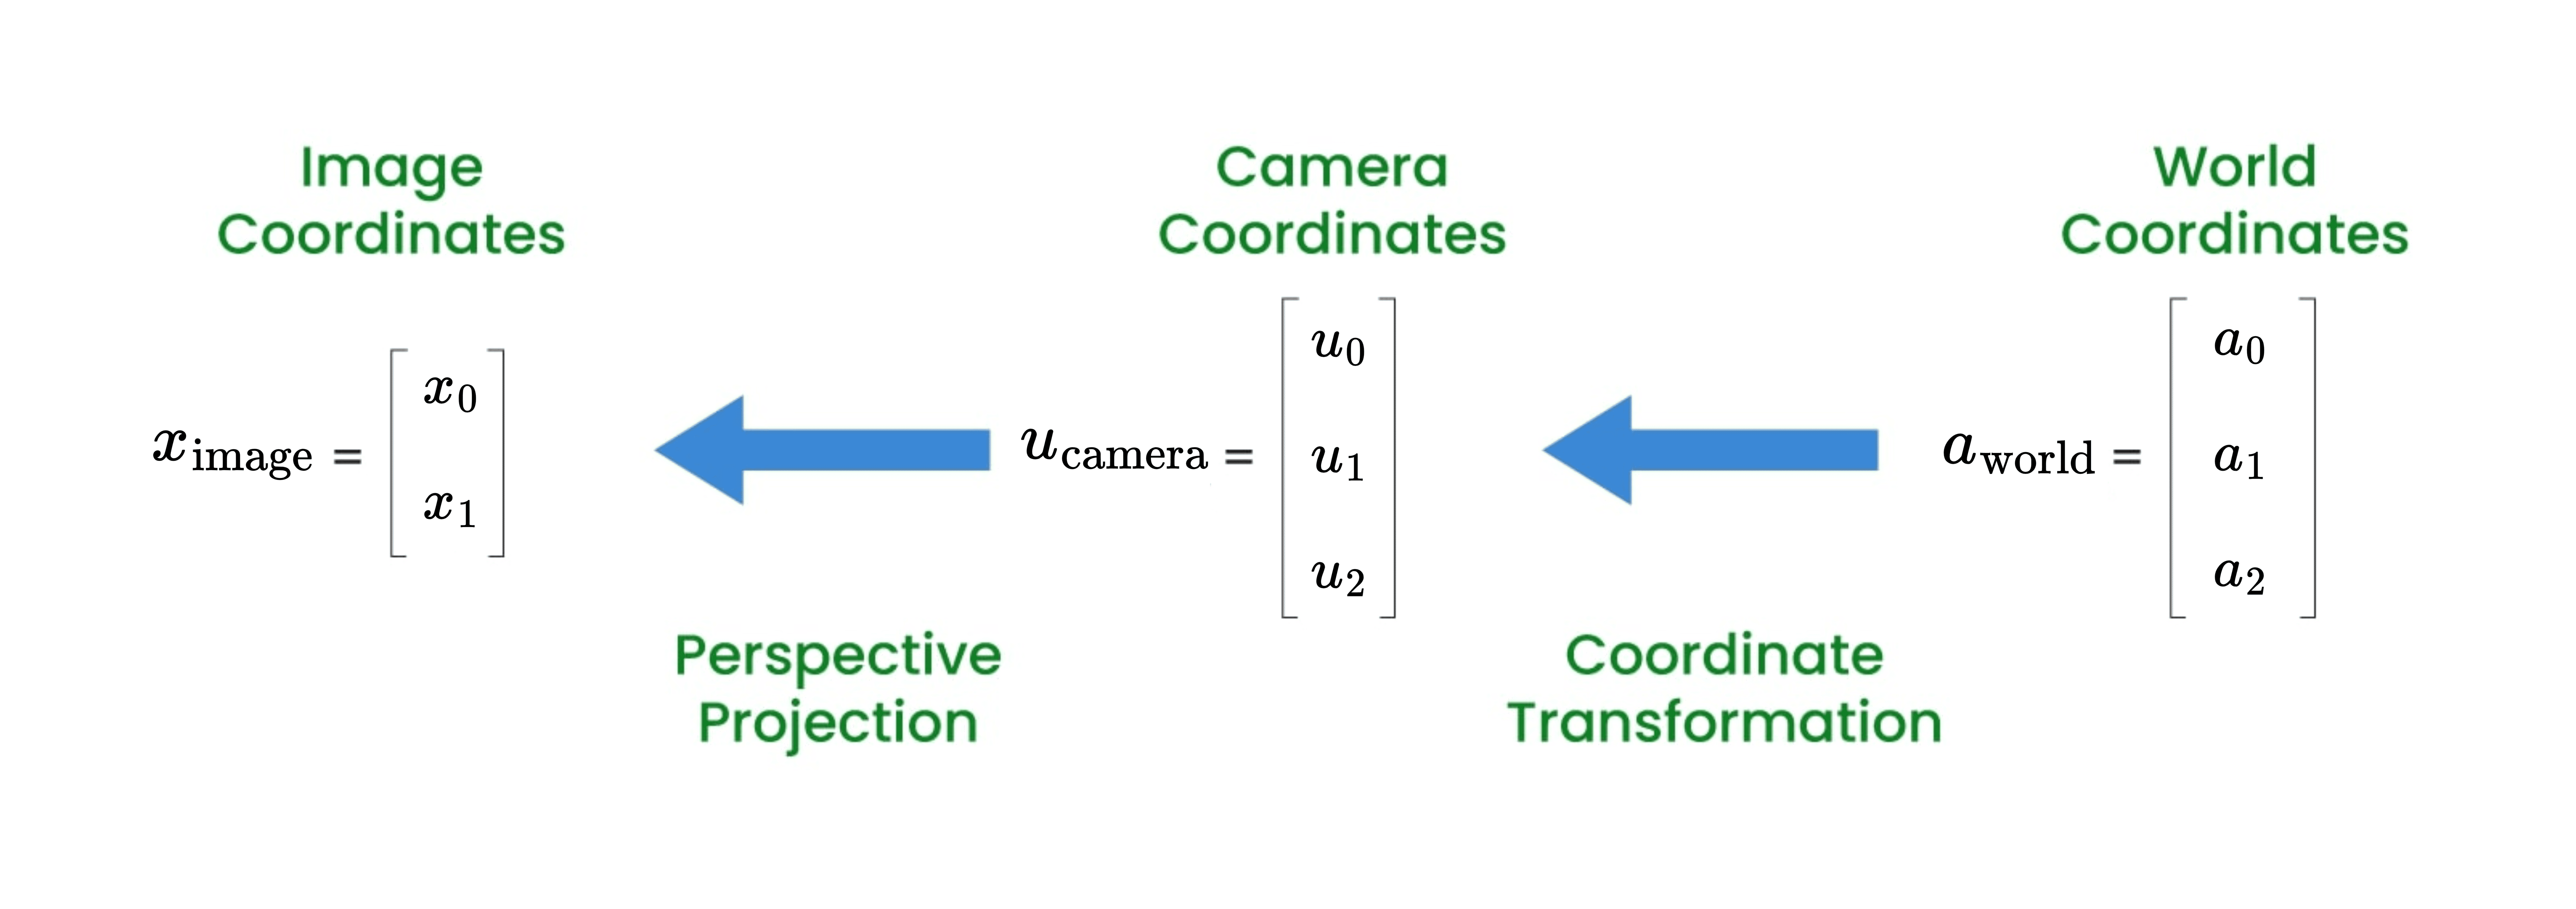
\includegraphics[width=0.45\textwidth]{assets/2.png}
	\caption{Process of projecting a 3D Gaussian into a 2D image plane.}
	\label{fig:2}
\end{figure}

We simply change coordinates using first a coordinate transformation (3D->3D) and then a perspective projection (3D->2D). The first is defined as:

\begin{equation}
	w_{camera} = E_{world}^{camera}a_{world} = Ra_{world} + T
\end{equation}

where R is a rotation matrix and T a translation vector. The perspective projection, instead, uses an \textbf{intrinsic matrix} (K) to project the 3D coordinates into 2D coordinates.

We have to apply this concept to the gaussians, which is a bit different. Since it is defined by a covariance matrix () and a mean vector (), the resulting distribution when transformed by the coordinate transformation () becomes:

\begin{equation}
	a \sim \mathcal{N}(\mu, \Sigma) \rightarrow \phi(a) \sim \mathcal{N}(W\mu + P, W\Sigma W^T) 
\end{equation}

After this step, we go to the \textbf{Ray Space}, a special non-linear transformation (3D->3D) that aligns the rays parallel to a coordinate axis making it easier to integrate along the ray \cite{zwicker2001ewa}.

\begin{figure}
	\centering
	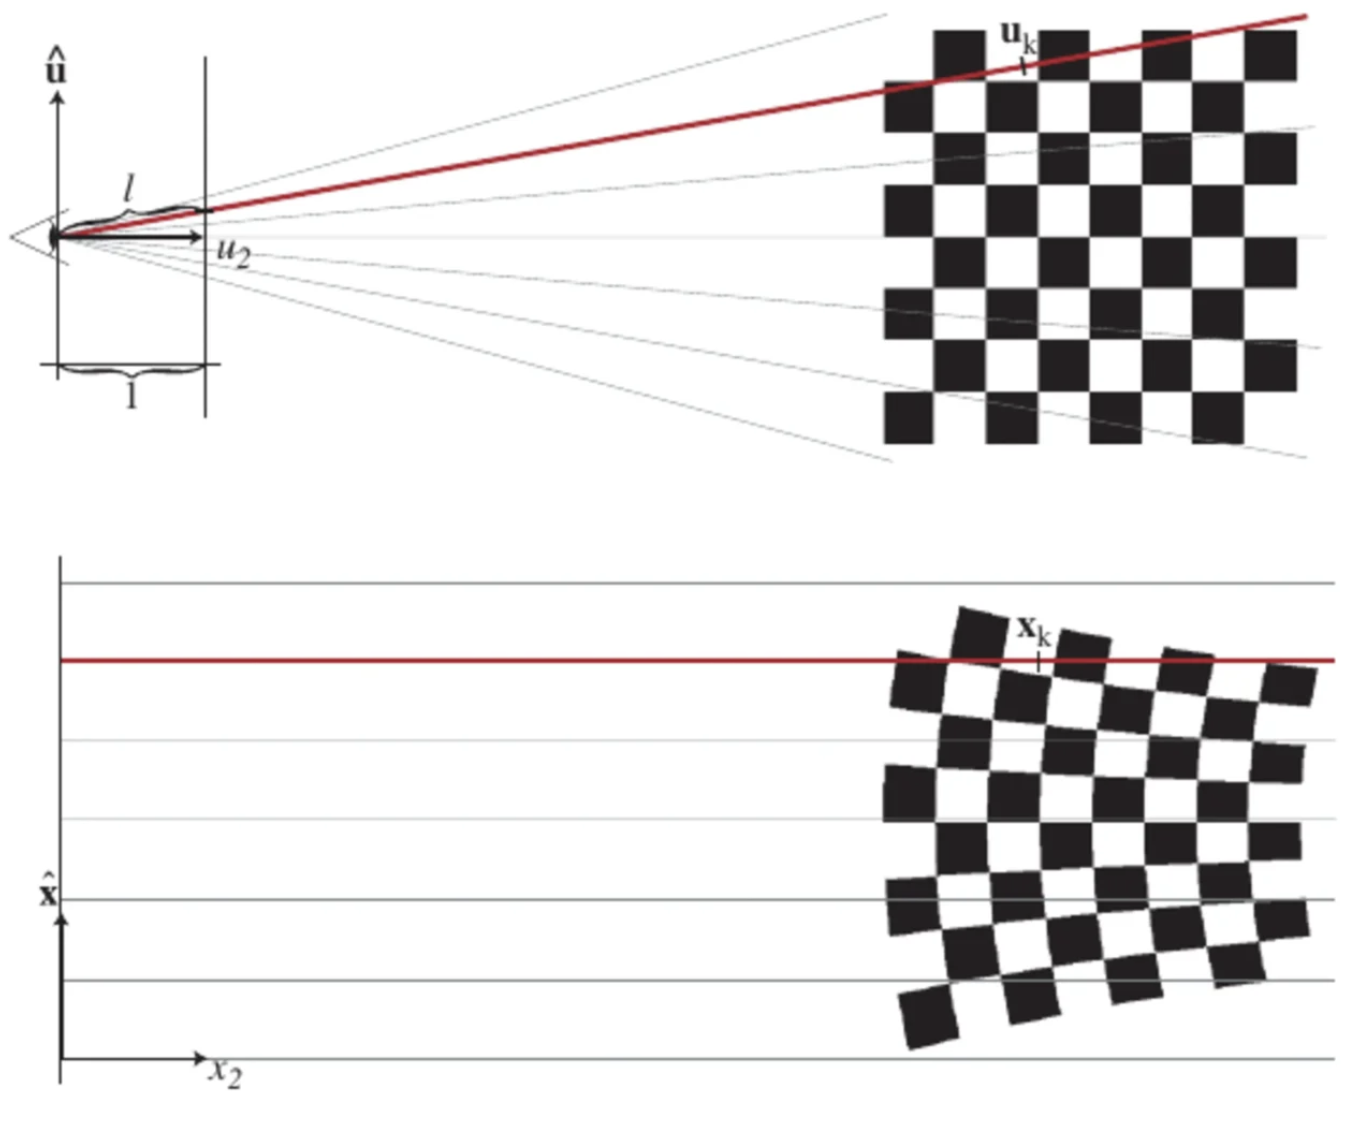
\includegraphics[width=0.45\textwidth]{assets/3.png}
	\caption{Process of transforming the 3D Gaussians into the Ray Space.}
	\label{fig:3}
\end{figure}

With this transformation, the mean vector becomes:

\begin{equation}
	m_{w_k}(u) = x_k + J_{w_k}(w - w_k), \quad J_{w_k} = \frac{\partial m_{w_k}}{\partial w(u_k)}
\end{equation}

while the covariance matrix becomes:

\begin{equation}
	\Sigma = \Sigma_{ray} = JW\Sigma W^TJ^T
\end{equation}

Now we can start understanding the algorithm:
\begin{enumerate}
	\item \textit{Input}: sparse point cloud from SfM + camera positions
	\item Each point is used to \textbf{initialize} the 3D gaussians
	\item Then \textbf{optimization} kicks in: we sample a camera position with image and project it into a 2D image plane. The image is rendered using that projection and a tile-based rasterizer, which is used to calculate the loss:
	\begin{equation}
		L = (1 - \lambda) L_1 + \lambda L_{D-SSIM}
	\end{equation}
	where the second component is an image similarity measure that uses Luminance, Contrast and Structural information.
	\item \textbf{Adaptive Density Control} adjusts dynamically number, density and parameters of the gaussians to accurately represent the 3D scene. It uses:
	\begin{enumerate}
		\item \textit{Pruning}: if opacity is too small or the gaussian is too large, it is removed
		\item \textit{Densification}: by Over-reconstruction, i.e., when regions are represented by too large or overlapping gaussians and in this case the gaussian is split in 2, or Under-reconstruction, i.e., the opposite and in this case we merge or duplicate the gaussians.
	\end{enumerate}
\end{enumerate}

\begin{figure}
	\centering
	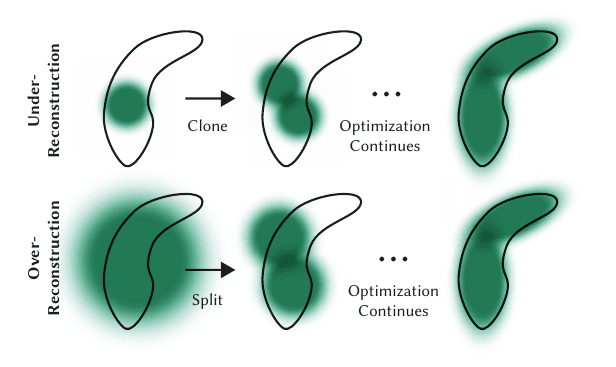
\includegraphics[width=0.45\textwidth]{assets/4.png}
	\caption{Process of optimization and adaptive density control in Gaussian Splatting.}
	\label{fig:4}
\end{figure}
Finally, \textbf{tile-based rasterization} is used to represent the 3D gaussians in a 2D image. The process is the one outlined above, with the single modification that the image is splitted in tiles so that parallelization and efficient use of GPUs can be done.

\subsection{Extensions of Gaussian Splatting}

Since the original 3DGS paper, a growing body of work has tried to address its main limitations, namely the poor geometric regularisation of the Gaussian cloud, the difficulty of recovering an explicit surface, and the restriction to reconstruction from existing multi-view captures. We discuss here three representative extensions that illustrate these directions.

A first line of work focuses on improving the \textbf{geometric quality} of the reconstruction. GaussianPro \cite{cheng2024gaussianpro} revisits the densification strategy of 3DGS, which relies on sparse SfM initialisation and tends to produce erroneous Gaussians in textureless regions. Inspired by classical Multi-View Stereo, it introduces a progressive propagation scheme that guides densification along the scene's surface structure, together with explicit plane constraints during optimisation. This yields more accurate geometry on large outdoor scenes, with reported PSNR improvements of around 1.15 dB over vanilla 3DGS on the Waymo dataset.

A second direction targets \textbf{surface and mesh extraction}. A limitation of 3DGS is that the optimised Gaussians are unstructured and do not directly provide an explicit surface, which is inconvenient for downstream tasks such as editing, animation or physically-based rendering. SuGaR \cite{guedon2024sugar} addresses this by adding a regularisation term that encourages Gaussians to align with the underlying surface, and then uses Poisson reconstruction to extract a triangle mesh from them. An optional refinement step binds Gaussians to the mesh and jointly optimises both through the Gaussian Splatting renderer, allowing mesh extraction in minutes instead of hours compared to SDF-based baselines, while preserving rendering quality.

Finally, Gaussian Splatting has been coupled with generative models to move from \textbf{reconstruction to 3D content creation}. DreamGaussian \cite{tang2024dreamgaussian} replaces the occupancy-based representations used in prior NeRF-based text- or image-to-3D pipelines with a generative 3DGS model, exploiting the progressive densification of Gaussians to speed up convergence. A companion mesh extraction and UV-space texture refinement stage produces textured meshes from a single image in roughly two minutes, about an order of magnitude faster than comparable NeRF-based approaches. This shows that the efficiency of 3DGS is not limited to multi-view reconstruction but also transfers to generative settings.

\section{Applications}

This section explores some of the diverse applications of 3D Gaussian Splatting (3DGS) as documented in the most recent literature from 2025 and 2026. As we will see in recent real-word tasks, 3DGS has evolved into a robust framework for geometric reconstruction and semantic scene understanding.

\subsection{Bird's-Eye-View (BEV) Representation and Autonomous Driving}

One of the most significant integrations of 3DGS is in autonomous driving pipelines. Instead of treating the perception as a black-box, recent frameworks like Splat2BEV \cite{splat2bev} use 3DGS as an intermediate representation. The approach allows the following:
\begin{itemize}
	\item \textit{Semantic segmentation}. It achieves state of the art results in identifying obstacles such as vehicles and pedestrians, and road elements like lanes by streaming information from vision foundation models into the Gaussian field. 
	\item \textit{Geometry-aligned representations}. Projecting 3D Gaussians into a top-down perspective (BEV space) to support downstream tasks like 3D object detection, path planning, etc.
	\item \textit{Simulation and sensor modeling}. It transforms large outdoors environments into editable Gaussian representations for effective rendering and also sensor simulation in testing environments.
\end{itemize}

In Splat2BEV, 3DGS is implemented as an intermediate representation by using what is called as Gaussian Generator ($G_\theta$), which is a feed-forward network that reconstructs 3D scenes from multi-view inputs. The generator first predicts a depth map for each perspective view, which is then unprojected into 3D space to establish the mean positions ($\mu$) of the Gaussian primitives. Additional attributes for each Gaussian, like opacity ($\sigma$) or covariance ($\Sigma$), are estimated by different prediction heads. Then, to enhance semantic understanding, a feature vector ($f$) that can be learned is attached to each Gaussian, allowing the framework to stream knowledge from vision foundation models (like DINO) directly into the Gaussian field. 
As mentioned earlier, Splat2BEV transforms the 3D Gaussians into a top-down BEV space. It does that by implementing a orthogonal projection, so the linear transformation preserves the geometric consistency of the scene when viewed form above. A Jacobian matrix ($J_{ortho}$) specifically designed for the BEV camera model is used to project each Gaussian into 2D space. Once the Gaussians are projected, a BEV feature map is integrated by using the differentiable rendering capability of 3DGS. The resulting BEV feature map is the direct input for BEV encoder and a segmentation head, which produce the final predictions for pedestrians, vehicles and road lanes.
The implementation of the framework follows a process of, first, pretraining the Gaussian generator to achieve accurate 3D reconstruction; then, the generator is frozen while the BEV encoder and segmentation heads are trained to interpret the 3DGS representation. Finally, the pipeline is fine-tuned, allowing gradients from the specific task's losses to flow back into the 3D Gaussian field to optimize the geometry and features for specific goals. \\


Another framework that focuses on the topic of autonomous driving is SSTD-GS \cite{sstdgs}, a self-supervised approach used for dynamic scene reconstruction. It enables:
\begin{itemize}
	\item \textit{Spatiotemporal deformation}. It achieves fine modeling of dynamic objects by predicting the motion properties of the Gaussian using a deformation field, capturing the movements without requiring manual 3D annotations.
	\item \textit{Uncertainty mask optimization}. It utilizes a self-supervised strategy to optimize both static and dynamic objects, improving the clarity of modeling in complex urban environments.
	\item \textit{Gaussian adaptive control}. It manages to suppress bad-quality densification caused by rendering errors, ensuring a robust scene reconstruction.
\end{itemize}

In the framework SSTD-GS, 3DGS is used as the core scene representation, augmented with a spatiotemporal deformation field to adress dynamic street scenes. SSTD-GS is built on normal Gaussian primitives, defined by their position ($\mu$), opacity ($\sigma$), covariance ($\Sigma$) and spherical harmonics ($SH$); and to enable the dynamic modeling, the framework adds two additional learnable parameters to each Gaussian: learnable velocity $v$ and a semantic attribute $f_{sem}$. $v$ encodes the motion characteristics of elements to learn deformations, and $f_{sem}$ ensures semantic consistency across frames so the objects do not disappear during the reconstruction.
The framework also implements a multi-head Gaussian decoder to transform the static Gaussians into dynamic ones. This is achieved by predicting the offset of the attributes, specifically four: position, pose, scale and appearance; as the decoder has four heads. Additionally, to supervise the 3D Gaussian field, the framework uses features based on 2D image from vision foundation models to generate a dynamic mask ($M$) for each frame. The velocity attributes of the Gaussians are mapped into a 2D velocity map, and the system then applies a loss function to ensure that Gaussians outside the mask (static ones) have velocity zero, separating dynamic and static elements.

\subsection{Bi-Modal and Thermal Mapping}

Gaussian attributes have such versatility that it has opened the door to multimodal applications, such as those that combine regular RGB photos with infrared (IR) images. This is what the BiNAR \cite{binar2026} framework proposes.
\begin{itemize}
	\item \textit{RGB-IR fusion}. The BiNAR framework allows the joint scene reconstruction of non aligned RGB and IR data. This can be applied to unmanned aerial night inspection and post-disaster thermal mapping, where thermal information is crucial, but lacks the resolution and texture of RGB images. It also achieves sub-pixel accuracy by having an average reprojection error of 0.242 px.
	\item \textit{Artifact suppresion}. The shared geometry of both modalities help remove artifacts, resulting in sharper edges and more consistent temperature gradients.
	\item \textit{Temperature modeling}. The authors of the framework created and released a new dataset that supports the recovery of real world temperature values at pixel level, aligned with the high resolution 3D geometry and textures from RGB.
\end{itemize}

BiNAR implements 3DGS as an Unified Gaussian Field that functions as a base for both RGB and IR modalities. This allows the model to process non-aligned data from the two types of sensors and produce aligned 3D reconstructions. The essence of BiNAR is the use of anisotropic 3D Gaussians that represent the scene's geometry at the same time it preserves the appearance characteristics of each sensor. All Gaussians share the same position, rotation and scale, ensuring cross-modal geometric consistency. This way, the 3D shape recognized in the RGB sensor matches the shape of the one in the IR spectrum. As the sensors have a lot of differences in terms of characteristics (color vs thermal info), each Gaussian has independent appearance parameters (opacity and Spherical Harmonics) for each type.

The pipeline for integrating Gaussian splatting starts by performing a pre-reconstruction of the RGB scene using COLMAP (general-purpose Structure-from-Motion and Multi-View Stereo pipeline) to estimate camera poses and generate a sparse point cloud. This provides the initial geometric anchors for the Gaussian distributions. For bimodal rendering, the framework uses the Mip-Splatting strategy to synthesize images from the Gaussian field, meaning now the system can render aligned RGB and IR views from any viewpoint. Moreover, BiNAR implements what is known as concurrent optimization, in which losses from both the RBG and IR images are propagated back through the pipeline at the same time to update the shared geometry and the specific appearance attributes.


\subsection{Urban Surveying and "In-the-Wild" Reconstruction}

Drones equipped with 3DGS-based frameworks like DroneSplat \cite{dronesplat2025} can be used for robust reconstruction in uncontrolled environments. This framework is useful for:
\begin{itemize}
	\item \textit{Eliminating dynamic distractors}. 3DGS methods can identify and mask moving objects (pedestrians or vehicles) in an adaptive way, producing static models of busy urban areas like streets and intersections.
	\item \textit{Geological and cultural preservation}. The maneuverability of drones combined with the representational capabilities of 3DGS can support geological investigations and the digital preservation of cultural sites that are difficult to access.
\end{itemize}

3DGS is applied in DroneSplat as the main representation for robust reconstruction from drone images. Same as in SSTD-GS, it uses the default Gaussian primitives, defined by position (center point, $\mu$), scaling ($S$), rotation ($R$), opacity ($\alpha$) and color ($f$). This framework's initialization process is more dense than the typical that relies on sparse point clouds, instead it uses a learning-based model (DUSt3R) to predict dense 3D points and confidence maps. Points are sampled based on their confidence and geometric features, the later being extracted using Fast Point Feature Histogram (FPFH) descriptors, ensuring the initial Gaussian primitives are placed in reliable areas.
Additionally, DroneSplat implements a special optimization strategy to mantain the geometric accuracy in regions with limited viewpoint overlap. First, the scene is divided into voxels, and bounds are forced on the Gaussians. Then, if a Gaussian's center or scale exceeds its voxel limits, it is flagged as "unconstrained", and its gradients are decayed exponentially. During the splitting or cloning process, new Gaussians are assigned only to neighboring empty voxels if the accumulated gradient excees a threshold and directs toward the voxel. Finally, voxels containing only a few Gaussians, or having a low average opacity, are removed, effectively eliminating artifacts.
To handle moving objects (like cars or pedestrians), the framework uses an adaptative masking method into the optimization loop. It calculates the mathematical expectation and variance of pixel residuals (L1 loss and D-SSIM) for every training frame, and then it adaptively adjusts a masking threshold so that pixels with residuals exceeding the threshold are identified as dynamic elements, excluding them from training. To also control distractors that temporarily stop (car at red light), the system uses the Segment Anything Model v2 (SAM2) to track "high-residual" candidates across frames. The global tracking results are combined with local masks to ensure the dynamic elements are eliminated consistenly from the static model.

\subsection{Super-Resolution and Sparse View Reconstruction}

Recent architectural improvements have augmented the applicability of 3DGS to areas or scenarios with limited and low-quality data. Frameworks like SR3R \cite{sr3r} can achieve it in the 3D scene, while other like MeshSplat \cite{meshsplat} are applied in 2D scenarios:
\begin{itemize}
	\item \textit{Super-resolution reconstruction}. SR3R can reconstruct high-resolution 3D scenes from low-resolution (LR) multi-view images, enabling high quality 3D models even when the hardware is limited.
	\item \textit{Sparse-view mesh generation}. Although not a 3D approach, MeshSplat uses 2D Gaussians as a link to integrate accurate surface geometry from very sparse input views, helping mesh reconstruction in computer vision tasks.
\end{itemize}

In a 3D super-resolution reconstruction in SR3R, 3DGS is implemented as the target high-resolution representation. The framework uses a neural network to predict high-resolution Gaussian attributes directly from sparse and low-resolution views that work as input. The way it works is the following: first a backbone generates a low-resolution "scaffold" and, then, SR3R takes the scaffold and upscales it into a high-resolution 3DGS representation; allowing the model to learn the 3D geometry and appearance from large-scale data.
To improve then the precision of the scene reconstructed, the framework implements Gaussian offset learning. That works by having the model predict spatial offsets for the Gaussian primitives, that help stabilize the reconstruction and sharpen the geometric details that are lost in low-resolution views. Additionally to the spatial offsets, SR3R implements a refinement of the features for the Gaussian attributes by refininig the appearance features of each Gaussian. This ensures the final high-resolution 3DGS representation catches the detailed textures and lightning effects.
What SR3R achieves in the end is a zero-shot generalization, producing high quality 3D models from limited and unseen data.

\subsection{Infrastructure Inspection and Digital Twins}

In the field of high fidelity modeling of industrial infrastructure, 3DGS has showed superior performance, especially in scenarios where traditional LiDAR struggles. Research on \cite{powergrid_3dgs} utilizes 3DGS to shed light on the following topics:
\begin{itemize}
	\item \textit{Power grid management}. Using 3DGS for the rapid 3D reconstruction of power transmission towers excelled at preserving fine structural details, like thin cables. These fine details are critical for fault detection and structural inspections.
	\item \textit{Asset lifecycle management}. By reducing the modeling time by $\sim 70\%$ compared to traditional methods, 3DGS seems to provide a technical foundation for digital twins, permitting documentation in virtual environments.
\end{itemize}

In \cite{powergrid_3dgs}, 3DGS is used as the reconstruction framework to make high-precision 3D models of power transmission towers. The 3DGS is implemented on top of a sparse point cloud that is generated through Structure from Motion (SfM). First RGM images captured by UAVs are processed using the COLMAP framework to estimate the camera poses and the sparse point cloud. Then, each 3D point is converted into the center of a learnable 3D Gaussian primitive that acts as a first distribution that accelerated the model's convergence and assures consistenty.
The towers are modeled with a lot of anisotropic Gaussians so the model can adapt to geometric features of changing scales, effectively allowing the model to represent robust structures but also fine details like thin cables. 
To later refine the model, a forward rendering and backward optimization loop is used. The mapping of the 3D world to a 2D image is done by transforming the primitives to the camera coordinate system, and the 2D covariance on the image plane is computed by a projection Jacobian matrix. Then a rendering pipeline collects the Gaussians influencing a pixel and performs alpha blending in depth order, synthetizing the final image.
There is also an adaptative density control method that handles the skeleton structure of power towers: if the current Gaussians are not enough to represent fine details, the system clones the existing primitives to add the details; and, if primitives are too large, it splits them into smaller and finer distributions to improve local resolution and capture fine geometric features. \\

Other authors also proposed a novel GS-enabled digital twin method \cite{digitaltwin_damage} for precise 3D damage visualization in civil infrastructures. This framework provides some key contributions:
\begin{itemize}
	\item \textit{Joint visualization and reconstruction}. Instead of first reconstructing and then visualizing the damages, this GS-based method incorporates the visualization directly into the reconstruction workflow by incorporating 2D segmentation results into the loss function, so the model is able to learn and correct segmentation errors while visualizing 3D damage simultaneously.
	\item \textit{Hierarchical reconstruction}. By using a hierarchical reconstruction strategy, the framework is able to conserve computational resources by first using low-resolution images for the initial overview of the structure. Then, only for regions with damage, high-resolution images are used to fine-tune the model, achieving a detailed reconstruction.
	\item \textit{Damage progression tracking}. It enables model updates  as the conditions of the structure evolve, so it permits the documentation of damage progression without requiring a full re-run of the scene reconstruction.
\end{itemize}

In \cite{digitaltwin_damage}, 3DGS is adapted to be semantically aware of damage in infrastructures, such as cracks and broken fragments. In this adapted 3DGS, each primitive is defined, as always by its position, covariance matrix (scale and orientation) and opacity, and the color is stored as RGB values enchanced by spherical harmonics to capture effects like shadows. The framework also allows regional adjustments, so it is possible to refine only the Gaussians related to specific damaged areas.
One of the innovation the framework proposes is the modification of the optimization objective in order to add 2D damage segmentation results directly into the 3D reconstruction. The raw images are not the only reference now, but the loss function compares the rendered outputs of the model against 2D segmented images, that are masks generated by deep learning models. With the new integration, the 3DGS multiview consistenct serves as a refinement process to supress inconsistencies that could be introduced by errors in the 2D segmented images. Basically the consensus across multiple viewpoints are prioritized over single instances in the 2D images. 
Furthermore, the framework implements a multi-scale strategy to balance efficiency and high-fidelity. First the framework generates a general and low-resolution model from low-resolution images to create the overall geometry. Secondly, when regions with suspected damage are identified, the framework separates the associated Gaussians through color filtering and projection validation. These Gaussians are updated using high-resolution images and the model can either be retrained or fine-tuned to capture the details of the cracks.
Finally, on the damage progression feature of this framework, new collected images are calibrated to the historical coordinate system of the model, and the framework renders synthetic views from the historical model from the same perspective as the new images. A pixel-wise comparison is performed between the synthetic masks and the new masks, so the system can highlight new damage. The new damage is then integrated into the existing 3D model through refinement of the relevant Gaussians, avoiding doing a full reconstruction of the structure.


\section{Experimentation}

To complement the literature review, we ran a small reproduction of the original 3D Gaussian Splatting pipeline on a single Mip-NeRF 360 scene. The code can be found in the following Colab notebook \footnote{https://colab.research.google.com/drive/1-AMqt-jT3cKZM5L3S8Mn0gAakdQHiVk6?usp=sharing}. The goal of this experiment is not to push state of the art, but to (i) get hands-on experience with the official implementation, (ii) verify that the results reported in \cite{kerbl20233dgs} are reproducible on a modest GPU, and (iii) provide concrete numbers (training time, model size, rendering speed) that put the qualitative descriptions of Section 3 in context.

\subsection{Setup}

We use the official reference implementation released by the authors of \cite{kerbl20233dgs} (\texttt{graphdeco-inria/gaussian-splatting}) without any modification, running it on a Google Colab notebook so that the experiment is fully reproducible from a browser. The notebook used for this experiment is available in the \texttt{experimentation/} folder of the project repository.

The hardware used is a single NVIDIA T4 GPU (16\,GB VRAM), which is the default Colab free-tier accelerator and a much weaker GPU than the NVIDIA A6000 used in the original paper. This allows us to verify that the method remains usable on entry-level hardware.

As discussed in Section 4, we evaluate on the \textbf{Mip-NeRF 360} dataset \cite{barron2022mipnerf360}, which is the de-facto benchmark for 3DGS. Among the nine scenes, we focus on \texttt{bonsai}, an indoor scene of about 290 photographs. Three considerations motivate this choice: it is one of the smallest scenes in the dataset, so the full 30k-iteration training run fits comfortably in the Colab time budget; it is contained, so the unbounded-background issues that affect the outdoor scenes are minimised; and it is reported in Table~1 of \cite{kerbl20233dgs}, which gives us a direct reference to compare against. Images are processed at half resolution (the \texttt{images\_2/} folder shipped with the dataset), and the official Mip-NeRF 360 train/test split is used (every 8\textsuperscript{th} view held out for testing).

\subsection{Protocol}

We follow exactly the protocol of \cite{kerbl20233dgs}: 30{,}000 optimisation iterations, the default Adaptive Density Control schedule, and the same composite $\mathcal{L}_1 + \mathcal{L}_{\textrm{D-SSIM}}$ loss with $\lambda = 0.2$. After training we use the \texttt{render.py} and \texttt{metrics.py} scripts shipped with the repository to render the test views and compute PSNR, SSIM and LPIPS. We additionally measure (a) the wall-clock training time, (b) the final number of 3D Gaussians (read directly from the saved \texttt{point\_cloud.ply}), and (c) the inference frame rate, obtained by re-rendering all test views in a tight loop after a short warm-up.

\subsection{Results}

Table~\ref{tab:exp_bonsai} reports our measurements alongside the reference numbers published in \cite{kerbl20233dgs} for the same scene.

\begin{table}[h]
    \centering
    \small
    \begin{tabular}{lcc}
        \toprule
        Metric                & Ours (Colab T4) & Reference \cite{kerbl20233dgs} \\
        \midrule
        PSNR ($\uparrow$)         & 32.44    & 32.20 \\
        SSIM ($\uparrow$)         & 0.948    & 0.941 \\
        LPIPS ($\downarrow$)      & 0.173    & 0.205 \\
        Training time (min)       & 67       & $\sim 30$ \\
        \# Gaussians ($10^6$)     & 1.07     & --- \\
        Inference FPS             & 42.9     & $\sim 150$ \\
        \bottomrule
    \end{tabular}
    \caption{3D Gaussian Splatting on the Mip-NeRF 360 \texttt{bonsai} scene. Our run uses a Colab T4 GPU; the reference numbers are reported in Table~1 of \cite{kerbl20233dgs} and were obtained on an NVIDIA A6000.}
    \label{tab:exp_bonsai}
\end{table}

\textbf{Quality.} The three quality metrics land essentially on top of the reference numbers: PSNR is $0.24$ dB higher, SSIM is $+0.007$, and LPIPS is $0.032$ lower (i.e.\ better) than \cite{kerbl20233dgs}. Since these metrics are scene-intrinsic and the official Mip-NeRF 360 train/test split is deterministic, the small differences are entirely consistent with the stochastic nature of Adaptive Density Control: each run of the optimiser converges to a slightly different cloud of Gaussians, but the rendering quality on the test views remains stable. The take-away is that the original 3DGS recipe is reproducible out of the box on a free Colab T4, with no hyper-parameter tuning, and that the published quality numbers are not an artifact of the high-end hardware used in the paper.

\textbf{Speed.} The two metrics that do depend on hardware tell a much less rosy story. Training takes $67$ minutes on the T4 against the $\sim 30$ minutes reported on an A6000 ($\sim 2.2\times$ slower), and inference runs at $42.9$ FPS against $\sim 150$ FPS ($\sim 3.5\times$ slower). This gap is in line with the raw compute difference between the two GPUs: the T4 delivers around $8$ TFLOPS of FP32 throughput against $\sim 38$ TFLOPS for the A6000, and has substantially less memory bandwidth. It is worth noting, however, that even at $42.9$ FPS the trained model is comfortably above the $30$ FPS interactive threshold, and on a free Colab GPU. This is the practical strength that the 3DGS paper advertises: even on entry-level hardware, the rendering pipeline remains real-time, while NeRF-style methods on the same scene would take seconds per frame.

\textbf{Model size.} The final model contains $\sim 1.07$ million Gaussians, which at the standard 59 floats per Gaussian corresponds to roughly $250$ MB on disk. This is a small enough footprint to be streamed over the network and visualised in a browser, and explains why an entire ecosystem of in-browser 3DGS viewers and editors has appeared since the original paper.

Overall, the experiment confirms the central message of \cite{kerbl20233dgs}: 3D Gaussian Splatting offers a very favourable quality-vs-cost trade-off compared to NeRF-based pipelines, and the trade-off scales gracefully down to commodity GPUs.

\section{Conclusions}

In this report, an insight into the evolution of 3D reconstruction pipelines has been provided, from the classical approaches into the focus of the assignment, 3D Gaussian Splatting. This method efficiently bridges the traditional approaches in the field with the recent neural networks, allowing for real-time rendering of scenes.

As discussed in previous sections, Gaussian Splatting is widely used in different applications, such as autonomous driving, thermal mapping through RGB and IR images or urban and wilderness reconstruction. This highlights its relevance in real world applications. In addition, the experiments carried out on Colab demonstrate the capabilities of this approach under limited hardware: while results are not as competitive as the original Gaussian Splatting paper reported in terms of speed, it is still a viable option for real-time rendering, in contrast with other reviewed approaches such as NeRF.

To summarise, 3D Gaussian Splatting manifests its relevance in the 3D multiscene reconstruction field, providing a balance between fidelity and efficiency, emerging as a state-of-the-art approach for real-time view synthesis.  

%----------------------------------------------------------------------------------------
%	 REFERENCES
%----------------------------------------------------------------------------------------

\printbibliography % Output the bibliography

%----------------------------------------------------------------------------------------

\end{document}
